\documentclass[numberindividually,nomasternumbers, numberwithin=lecture]{hrflecture}
\renewcommand*{\sectionformat}{\textsection\thesection\autodot\enskip}
\addtokomafont{section}{\mdseries}

\subject{Vorlesungsmitschrift}
\title{AGLA \texorpdfstring{\Romannum{2}}{2}}
\subtitle{Prof.~Dr.~Damaris~Schindler}
\date{Auf dem Stand vom \today}
\author{Henry Ruben Fischer}

\begin{document}
\maketitle

\newpage
\textbf{Disclaimer}
\vspace{1cm}

Nicht von Professor Schindler durchgesehene Mitschrift, keine Garantie auf Richtigkeit ihrerseits.

\newpage
\tableofcontents
\newpage

% some more adjustments
\makeatletter
\renewtheorem{satz}[lemma]{Satz}
\def\thm@fmt@hyplabel@ii#1.#2.#3{#3} % I don't quite understand this
\makeatother

% Begin of lectures
% !TEX root = ./Vorlesungsmitschrift AGLA 2.tex 
\chapter{Affine Geometrie}
\lecture{1}{Di 21.04. 10:15}{}
\section{Was ist ein affiner Raum?}
\begin{beispiel}[aus der AGLA \Romannum{1}]
    \( \reals^2, \reals^3 \). 
    In diesen Räumen gibt es einen ausgezeichneten \enquote{Usprung}.
\end{beispiel}
\begin{frage*}
    Wie könne wir eine affine Ebene / affine Röume modellieren, wobei alle Punkte gleichberechtigt sind?
\end{frage*}
\begin{idee*}
    Verwende affine Unterräume.
\end{idee*}
\begin{beispiel}\label{affiner_unterraum}
    Sei \( K \) ein Körper, \( V \) ein \( K \)-Vektorraum, \( W\subseteq V \) ein Untervektorraum und \( v\in V \). 
    Wir nennen \( X=v+W \) einen affinen Unterraum von \( V \). 
    \( X \) ist im Allgemeinen selbst kein Vektorraum unter der Addition in \( V \), aber \( W \) \enquote{operiert} auf \( X \).
    \begin{figure}[H]
        \centering
        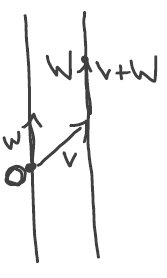
\includegraphics[width=0.2\linewidth]{figures/affiner_unterraum}
        \label{fig:affiner_unterraum}
    \end{figure}
    
    Für \( w\in W \) definieren wir die Abbildung
    \begin{align*}
        \tau_w\maps \begin{aligned}[t] 
            X&\to X\\
            p &\mapsto p+w.
        \end{aligned}
    \end{align*}
    \begin{figure}[H]
        \centering
        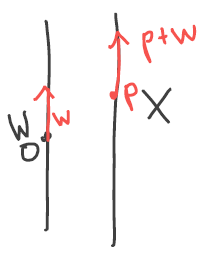
\includegraphics[width=0.2\linewidth]{figures/tau_w}
        \label{fig:tau_w}
    \end{figure}
    Sei
    \begin{align*}
        \Bij(X)=\Set{f\maps X\to X, f \text{ ist bijektiv}}.
    \end{align*}
    Dann ist \( \tau_w\in \Bij(X) \) für alle \( w\in W \).
\end{beispiel}
\begin{bemerkung*}
    \( \Bij(X) \) ist eine Gruppe unter Verkettung von Abbildung. 
    Wir erhalten eine Abbildung
    \begin{align*}
        \tau\maps \begin{aligned}[t] 
            W &\to \Bij(X)\\
            w &\mapsto \tau_w.
        \end{aligned}
    \end{align*}
\end{bemerkung*}
\begin{lemma}
    Die Abbildung \( \tau \) ist ein Gruppenhomomorphismus.
\end{lemma}
\begin{proof}
    Seien \( w, w' \in W \)
    Dann
    \begin{align*}
        \tau_w\circ \tau_{w'}\maps \begin{aligned}[t] 
            X &\to X\\
            p &\mapsto p+\underbracket{w'+w},
        \end{aligned}
    \end{align*}
    also
    \begin{align*}
        \tau(w)\circ \tau(w')=\tau_w\circ \tau_{w'}=\tau_{w+w'}=\tau(w+w').
    \end{align*}
    
\end{proof}
Es gilt noch mehr:

\textcolor{Turquoise}{für \( p, q \in X \)} besteht genau ein \( w\in W \) mit \( \tau_w(p)=q \).

\begin{figure}[H]
    \centering
    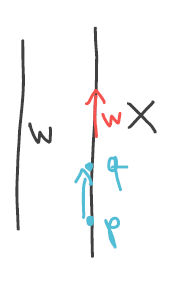
\includegraphics[width=0.2\linewidth]{figures/tau_w_bijektion}
    \label{fig:tau_w_bijektion}
\end{figure}

\section*{Gruppenoperationen}
\begin{beispiel}\label{d_3}
    Betrachte ein gleichseitiges Dreieck \( D \) und Spiegelungen / Drehungen die \( D \) auf sich selbst abbilden.

    \begin{figure}[H]
        \centering
        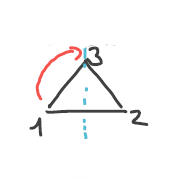
\includegraphics[width=0.2\linewidth]{figures/d_3}
        \label{fig:d_3}
    \end{figure}
    Diese formen eine Gruppe (welche?) und \enquote{operieren} auf \( D \).
\end{beispiel}
\begin{definition}
    Sei \( X \) eine Mege und \( G \) eine Gruppe. 
    Eine Operation von \( G \) auf \( X \) ist ein Homomorphismus von Gruppen
    \begin{align*}
        \tau\maps \begin{aligned}[t] 
            G&\to \Bij(X)\\
            g&\mapsto \tau_g.
        \end{aligned}
    \end{align*}
\end{definition}
\begin{bemerkung*}
    \( \tau \) ist ein Homomorphismus \dh \tforall \( g, g' \in G \)
    \begin{align*}
        \tau_g\circ \tau_{g'}=\tau_{gg'}.
    \end{align*}
    
    Für \( x\in X \) nennen wir
    \begin{align*}
        G(x)=\Set{\tau_g(x)|g\in G}
    \end{align*}
    die Bahn von \( x \) unter \( G \).
\end{bemerkung*}
\begin{beispiel}\label{operation:beispiele}
    \begin{eigenschaftenenumerate}
        \item \label{operation:beispiele:linkstranslation} Sei \( G \) eine Gruppe und \( X=G \) die Linkstranslation \( l\maps \begin{aligned}[t] 
            G&\to \Bij(G)\\
            g&\mapsto l_g
        \end{aligned} \) mit \( l_g(x)=gx \quad\forall x\in G \) ist eine Gruppenoperation von \( G \) auf sich selbst.
        
        \item \label{operation:beispiele:konjugation}\begin{align*}
            k\maps \begin{aligned}[t] 
                G &\to \Bij(G)\\
                g &\mapsto kg
            \end{aligned}
        \end{align*}
        mit \( k_g(x)=gx\inv{g} \quad\forall x\in G \) ist eine Gruppenoperation.
    \end{eigenschaftenenumerate}
\end{beispiel}
\thref{operation:beispiele}~\ref{operation:beispiele:konjugation}
\begin{frage*}
    Sei \( \tau\maps G\to \Bij(x) \) eine Gruppenoperation, \( x,y\in X \). 
    Wann gibt es ein \( g\in G \) mit \( \tau_g(x)=y \)?
    \begin{figure}[H]
        \centering
        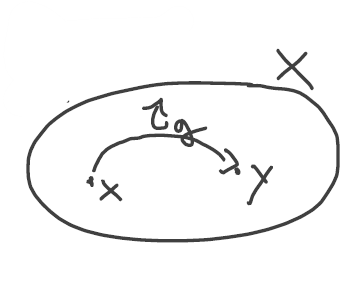
\includegraphics[width=0.5\linewidth]{figures/einfach_transitiv}
        \label{fig:einfach_transitiv}
    \end{figure}
    
\end{frage*}

\begin{definition*}
    Sei \( \tau\maps G\to \Bij(X) \) eine Gruppenoperation von \( G \) auf \( X \). 
    Wir nennen \( \tau \) \emph{einfach transitiv}, wenn \tforall \( x,y\in X \) \emph{genau ein} \( g\in G \) besteht mit
    \begin{align*}
        \tau_g(x)=y.
    \end{align*}
\end{definition*}
\begin{beispiel*}
    \begin{itemize}
        \item Die Gruppenoperation aus \thref{d_3} ist \emph{nicht} einfach transitiv
        \begin{figure}[H]
            \centering
            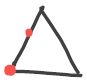
\includegraphics[width=0.2\linewidth]{figures/d_3_nicht_einfach_transitiv}
            \label{fig:d_3_nicht_einfach_transitiv}
        \end{figure}
        
        \item Die Linkstranslation aus \thref{operation:beispiele}~\ref{operation:beispiele:linkstranslation} ist immer einfach transitiv.
    \end{itemize}
\end{beispiel*}
Zurück zum \thref{affiner_unterraum} (\( V \) \( K \)-Vektorraum, \( W\subseteq V \) Untervektorraum, \( v\in V \), \( X=v+W \))

Wir haben Translationen definiert
\begin{align*}
    \tau\maps \begin{aligned}[t] 
        W&\to \Bij(X)\\
        x&\mapsto \tau_w
    \end{aligned}
\end{align*}
mit \( \tau_w\maps X\to X \), \( p\mapsto p+w \). 
\( \tau \) ist eine einfach transitive Gruppenoperation von \( W \) auf \( x \).

\begin{figure}[H]
    \centering
    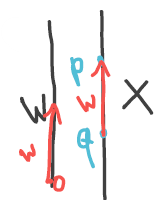
\includegraphics[width=0.2\linewidth]{figures/affiner_unterraum_einfach_transitive_gruppenoperation}
    \label{fig:affiner_unterraum_einfach_transitive_gruppenoperation}
\end{figure}

\begin{definition*}
    Sei \( K \) ein Körpr. 
    Ein affiner Raum über \( K \) ist ein Tripel \( (X, T(X), \tau ) \) mit
    \begin{itemize}
        \item \( X\neq \emptyset \) eine Menge 
        \item \( T(X) \) ein \( K \)-Vektorraum 
        \item \( \tau\maps T(x)\to \Bij(X) \) eine einfach transitive Gruppenoperation
    \end{itemize}
\end{definition*}
\begin{konvention*}
    \( X=\emptyset \) ohne Spezifikation von \( T(X) \), \( \tau \) nennen wir auch einen affinen Raum.
\end{konvention*}
\begin{figure}[H]
    \centering
    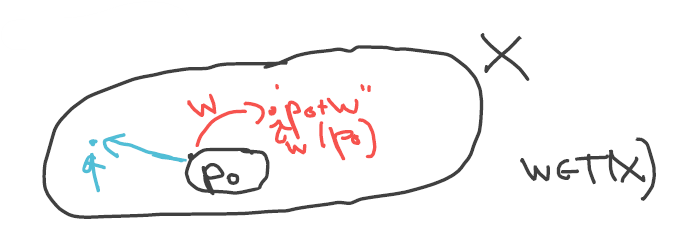
\includegraphics[width=0.5\linewidth]{figures/affiner_raum}
    \label{fig:affiner_raum}
\end{figure}
\begin{definition*}
    Sei \( (X,T(X),\tau) \) in affiner Raum über einem Körper \( K \). 
    Dann nennen wir \( \dim_K T(X) \) die Dimension von \( X \), schreiben auch \( \dim X \).
     
    Ist \( \dim X=1 \) \bzw \( \dim X=2 \), dann nennen wir \( X \) eine affine Gerade \bzw affine Ebene.
\end{definition*}

Sei \( (X, T(X), \tau) \) in affiner Raum, \( p,q\in X \). Dann \( \existsone t\in T(X) \) mit \( \tau_t(p)=q \).

\textcolor{Turquoise}{Schreibe \( \vv{pq}=t\in T(X) \) als \( \tau_{\vv{pq}}(p)=q \).}
\begin{figure}[H]
    \centering
    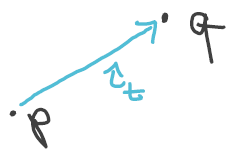
\includegraphics[width=0.2\linewidth]{figures/vektornotation}
    \label{fig:vektornotation}
\end{figure}
Wir erhalten eine Abbildung
\begin{align*}
    X\times X&\to T(X)\\
    (p,q)&\mapsto \vv{pq}.
\end{align*}
\begin{frage*}
    Welche Eigenschaften hat die Abbildung \( (p,q)\mapsto \vv{pq} \) in einem allgemeinen affinen Raum?
\end{frage*}
\begin{lemma}\label{vektoren_funzen_richtig}
    Sei \( X \) ein affiner Raum, \( p,q,r\in X \). Dann gilt \( \vv{pq}+\vv{qr}=\vv{pr} \).
\end{lemma}
\begin{figure}[H]
    \centering
    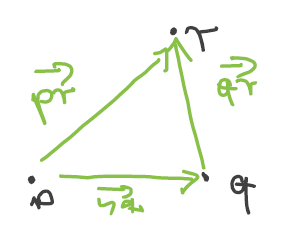
\includegraphics[width=0.3\linewidth]{figures/vektoren_funzen_richtig}
    \label{fig:vektoren_funzen_richtig}
\end{figure}
\begin{proof}
    \( \tau\maps T(X)\to \Bij(X) \) ist ein Homomorphismus. 
    Also gilt \( \tau_{\vv{qr}}\circ \tau_{\vv{pq}}=\tau_{\vv{pq}+\vv{qr}} \). 
    Es gilt damit \( \tau_{\vv{pq}+\vv{qr}}(p)=r \). 
    Also \( \vv{pq}+\vv{qr}=\vv{pr} \).    
\end{proof}

\section{Affine Abbildungen}
Seien \( V,W \) \( K \)-Vektorräume.
In der AGLA \Romannum{1}: lineare Abbildungen
\begin{align*}
    F\maps V\to W,
\end{align*}
\dh \( F \) respektiert die Vektorraum-Struktur
\begin{align*}
    F(v_1+v_2)=F(v_1)+F(v_2)\quad\forall v_1,v_2\in V\\
    F(\lambda v)=\lambda F(v)\quad \forall\lambda\in K \forall v \in V.
\end{align*}
\begin{frage*}
    Was sind natürliche Abbildungen zwischen affinen Räumen?
\end{frage*}
Seien \( X, Y \) affine Räume über einem Körper \( K \).

Seien \( X, Y \) affine Räume über einem Körper \( K \)
\begin{figure}[H]
    \centering
    \includegraphics[width=0.8\linewidth]{figures/affine_Abbildungen}
    \label{fig:affine_Abbildungen}
\end{figure}
\begin{align*}
    \textcolor{Turquoise}{\vertrelate{\vertni}{T(X)}{\vv{pq}}\rightsquigarrow\vertrelate{\vertni}{T(Y)}{\vv{f(p)f(q)}}}.
\end{align*}
\begin{definition*}
    Wir nennen eine Abbildung \( f\maps X \to Y \) affin, wenn s eine \( K \)-lineare Abbildung \( F\maps T(X)\to T(Y) \) gibt, sodass \tforall \( p,q\in X \) gilt
    \begin{align*}
        \vv{f(p)f(q)}=F(\vv{pq}).
    \end{align*}
\end{definition*}
\begin{bemerkung*}
    \begin{eigenschaftenenumerate}
        \item Es gibt im Allgemeinen verschiedene affine Abbildungen \( f\maps X \to Y \), die zur gleichen linearen Abbildung \( F\maps T(X)\to T(Y) \) gehören.
        \item Sei \( p_0 \in X \) fest und \( f\maps X \to Y \) affin.
        
        Für \( q\in X \) gilt
        \begin{align*}
            f(q)\begin{aligned}[t] 
                &=\tau_{\vv{f(p_0)f(q)}}(f(p0))\\
            &=\tau_{F(\vv{p_0 q})}(f(p0)).
            \end{aligned}
        \end{align*}
        Also bestimmen \( f(p_0) \) und \( F \) zusammenen die Abbildung \( f\maps X\to Y \).
    \end{eigenschaftenenumerate}


\end{bemerkung*}
\begin{beispiel*}
    Seien \( V,W \) \( K \)-Vektorräume
    \begin{align*}
        X=(V,V,\tau),\quad Y=(W,W,\tau).
    \end{align*}
    Eine affine Abbildung \( f\maps V\to W \) ist eindeutig bestimmt durch \( f(0) \) und eine lineare Abbildung \( F\maps V\to W \). Es gilt
    \begin{align*}
        f(v)=\textcolor{Goldenrod}{f(0)}+\textcolor{LimeGreen}{F(v)}\quad\forall \textcolor{LimeGreen}{v} \in V.
    \end{align*}
\end{beispiel*}
\begin{figure}[H]
    \centering
    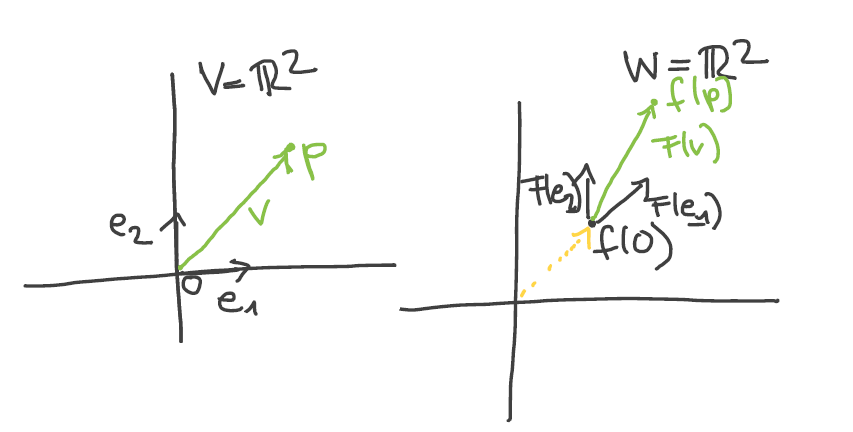
\includegraphics[width=0.7\linewidth]{figures/affine_abbildungen_vektorraeume}
    \label{fig:affine_abbildungen_vektorraeume}
\end{figure}
\begin{bemuebung*}
    Eine affine Abbildung \( f\maps X \to Y \) ist genau dann injektiv \bzw surjektiv \bzw bijektiv, wenn die zugehörige Abbildung \( F\maps T(X)\to T(Y) \).
\end{bemuebung*}
\begin{definition*}
    Wir nennen eine bijektive affine Abbildung \( f\maps X \to Y \) eine Affinität.
\end{definition*}
\section*{Affine Unterräume}
\begin{beispiel*}[\( \reals^2 \) als Vektorraum.]
    Untervektorräume von \( \reals^2 \) sind \( \emptyset \), \( \zeroset \), \( \reals^2 \) und Geraden durch \( 0 \).
    \begin{figure}[H]
        \centering
        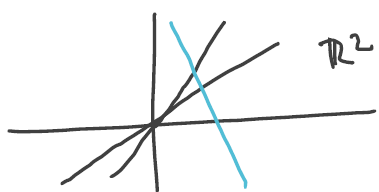
\includegraphics[width=0.4\linewidth]{figures/untervektorraeume_r2}
        \label{fig:untervektorraeume_r2}
    \end{figure}
    Betrachte nun \( \reals^2 \) als affinen Raum.
    \begin{figure}[H]
        \centering
        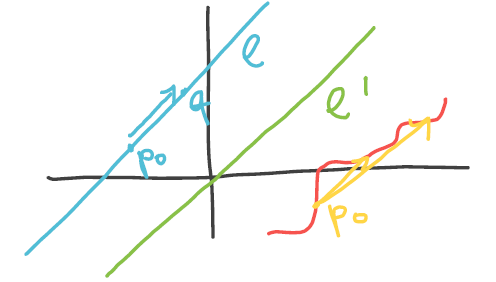
\includegraphics[width=0.5\linewidth]{figures/affine_unterraeume_r2}
        \label{fig:affine_unterraeume_r2}
    \end{figure}
    \begin{idee*}
        Wir wollen \( l \) und \( l' \) als affine Unterräume von \( \reals^2 \) definieren, da die Verschiebung von \( l, l' \) jeweils Untervektorräume von \( \reals^2 \) sind.
    \end{idee*}
\end{beispiel*}

\begin{definition*}
    Sei \( (X,T(X), \tau) \) in affiner Raum und \( Y\subseteq X \). Wenn es einen Punkt \( p_0 \in Y \) gibt, sodass
    \begin{align*}
        T(Y)\definedas \Set{\vv{p\circ q}\in T(X), q\in Y}
    \end{align*}
    ein Untervektorraum von \( T(X) \) ist, dann nennen wir \( Y \) einen affinen Unterraum von \( X \).
\end{definition*}
\begin{lemma}
    Sei \( Y\subseteq X \) ein affiner Unterraum eines affinen Raumes \( (X,T(X),\tau) \). Dann gilt
    \begin{align*}
        T(Y)=\Set{\vv{pq}\in T(X), q\in Y}
    \end{align*}
    für jedes beiliebigen Punkt \( p\in Y \).
\end{lemma}
\begin{proof}
    Sei \( p_0\in Y \) ein fester Punkt mit
    \begin{align*}
        T(Y)=\Set{\vv{p_0 q}\in T(X), q \in Y}
    \end{align*}
    Untervektorraum von \( T(X) \).
    Dann gilt für \( p \in Y \)
    \begin{align*}
        \Set{\vv{pq}|q\in Y}=\vv{pp_0}+\Set{\vv{p_0 q}| q\in Y}=\vertrelate{\vertni}{T(Y)}{\vv{p p_0}}+ T(Y)=T(Y),
    \end{align*}
    da \( \vv{p p_0}=-\vv{p_0 p}\in T(Y) \).
    
\end{proof}
\begin{definition*}
    Sei \( Y\subseteq X \) ein affiner Unterraum. Wir nennen \( \dim_K T(Y) \) die Dimension von \( Y \) und schreiben 
    \begin{align*}
        \dim Y=\dim_K T(Y).
    \end{align*}
\end{definition*}



% !TEX root = ./Vorlesungsmitschrift AGLA 2.tex  
\lecture{Fr 24.10. 10:15}{}
\section{Durchschnitt und Verbindung affiner Räume}
\begin{frage*}
    Sei \( X \) ein affiner Raum, \(    Y_1, Y_2 \) affine Unterräume von \( X \). Sind \( Y_1\cap Y_2, Y_1\cup Y_2 \) auch affine Unterräume von \( X \)?
    \begin{figure}[H]
        \centering
        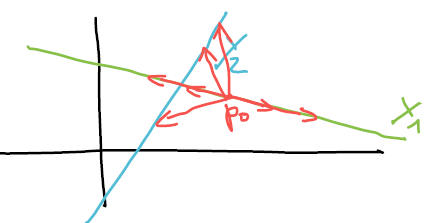
\includegraphics[width=0.5\linewidth]{figures/verbindung_affine_raeume}
        \caption*{\( X=\reals^2 \)}
        \label{fig:verbindung_affine_raeume}
    \end{figure}
\end{frage*}
\begin{lemma}\label{schnittraum:translationen}
    Sei \( X \) ein affiner Raum, \( Y_i \), \( i\in I \), eine Familie von affinen Unterräumen von \( X \).

    Dann ist \( Y\definedas \bigcap_{i\in I} Y_i \) ein affiner Unterraum von \( X \).

    Wenn \( Y\neq \emptyset \), dann gilt
    \begin{align*}
        T(Y)=\bigcap_{i\in I}T(Y_i).
    \end{align*}
\end{lemma}
\begin{proof}
    Falls \( Y=\emptyset \): \checkmark

    Wir nehmen also an \( Y\neq \emptyset \).
    Sei \( p_0\in Y \).
    Dann gilt:
    \begin{align*}
        T(Y)\begin{aligned}[t] 
            &=\Set{\underrelate{\textcolor{Goldenrod}\vertni}{\textcolor{Goldenrod}{T(X)}}{\vv{p_0 q}},q\in \bigcap_{i\in I}Y_i}\\
            &=\bigcap_{i\in I}\textcolor{LimeGreen}{\underbrace{\Set{\vv{p_0 q}, q\in Y_i}}_{=T(Y_i)}}\\
            &=\bigcap_{i\in I}T(\explain[big]{\text{Untervektorräume von \( T(X) \)}}{Y_i}).
        \end{aligned}
    \end{align*}
    Also ist \( T(Y) \) ein Untervektorraum von \( T(X) \) und \( T(Y)=\bigcap_{i\in I}T(Y_i) \).
\end{proof}
\begin{bemerkung*}
    In obiger Notation ist \( \bigcup_{i\in I}Y_i \) im Allgemeinen kein affiner Unterraum von \( X \).
\end{bemerkung*}
\begin{frage*}
    Finde den \enquote{kleinsten} affinen Unterraum von \( X \), der \( \bigcup_{i\in I}Y_i \) enthält! (\zb \( X\supseteq \bigcup_{i\in I} Y_i\), aber \( X \) ist im Allgemeinen nicht \enquote{minimal}).
\end{frage*}
\begin{definition*}
    Sei \( X \) ein affiner Raum, \( Y_i \), \( i\in I \) affine Unterräume von \( X \). Wir nennen
    \begin{align*}
        \bigcap_{\mathclap{\substack{Y\subseteq X \text{ aff.\ Unterraum}\\
         \bigcup_{i\in I}Y_i\subseteq Y}}}Y
    \end{align*}
    den \emph{Verbindungsraum} der affinen Unterräume \( Y_i \), \( i\in I \). Schreibe \( \bigvee_{i\in I}Y_i \).
\end{definition*}
\begin{beispiel*}
    \begin{figure}[H]
        \centering
        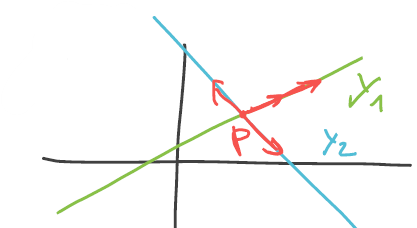
\includegraphics[width=0.5\linewidth]{figures/verbindungsraum_zwei_geraden}
        \caption*{\( X=\reals^2 \), \( Y_1\vee Y_2=X \), \textcolor{OrangeRed}{\( Y=Y_1\vee Y_2 \), \( T(Y)=T(Y_1)+T(Y_2) \)}.}
        \label{fig:verbindungsraum_zwei_geraden}
    \end{figure}
    
\end{beispiel*}

\begin{frage*}
    Wie kann man im Allgemeinen \( T(Y_1\vee Y_2) \) aus \( T(Y_1),T(Y_2) \) bestimmen?
\end{frage*}
\begin{lemma}\label{verbindungsraum:translationen}
    Sei \( X \) ein affiner Raum, \( Y_1,Y_2\neq\emptyset \) affine Unterräume von \( X \).
    \begin{eigenschaftenenumerate}
        \item \label{verbindungsraum:translationen:schnitt_nicht_leer}Sei \( Y_1\cap Y_2\neq \emptyset \).
        Dann gilt
        \begin{align*}
            T(Y_1\vee Y_2)=T(Y_1)+T(Y_2).
        \end{align*}
        
        \item \label{verbindungsraum:translationen:schnitt_leer}Sei \( Y_1\cap Y_2=\emptyset \), \( p_1\in Y_1, p_2\in Y_2\) und \( Y=p_1\vee p_2 \).
        
        Dann gilt:
        \begin{align*}
            T(Y_1\vee Y_2)=(T(Y_1)+T(Y_2))\oplus T(Y).
        \end{align*}
    \end{eigenschaftenenumerate}
\end{lemma}
\begin{proof}
    \begin{proofdescription}
        
        \item[\ref{verbindungsraum:translationen:schnitt_nicht_leer}]
        \begin{figure}[H]
            \centering
            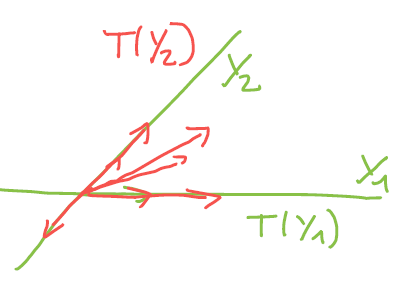
\includegraphics[width=0.5\linewidth]{figures/verbindungsraum_translationen_schnitt_nicht_leer}
            \label{fig:verbindungsraum_translationen_schnitt_nicht_leer}
        \end{figure}
         Sei \( p\in Y_1\cap Y_2 \). Dann gilt
         \begin{align*}
             T(Y_1)\cup T(Y_2)\begin{aligned}[t] 
                &=\Set{\vv{pq}|q\in Y_1\cup Y_2}\\
                &\subseteq T(Y_1\vee Y_2),
             \end{aligned}
         \end{align*}
         also \( T(Y_1)+T(Y_2)\subseteq T(Y_1\vee Y_2) \).

         Sei \( Y=\Set{\tau_t(p)|t\in T(Y_1)+T(Y_2)} \).
         Dann ist \( Y \) affiner Unterraum von \( X \) mit \( Y_1\cup Y_2\subseteq Y \), also \( Y_1\vee Y_2\subset Y \), also \( Y_1\vee Y_2\subseteq Y \). Also gilt
         \begin{align*}
             T(Y_1\vee Y_2)\subseteq T(Y)=T(Y_1)+T(Y_2).
         \end{align*}
         
         Also \( T(Y_1\vee Y_2)=T(Y_1)+T(Y_2) \).
         
         \item[\ref{verbindungsraum:translationen:schnitt_leer}]
         \( Y_1\cap Y_2=\emptyset \), \( p_1\in Y_1 \), \( p_2\in Y_2 \), \( Y=p_1\vee p_2 \).
         \begin{figure}[H]
             \centering
             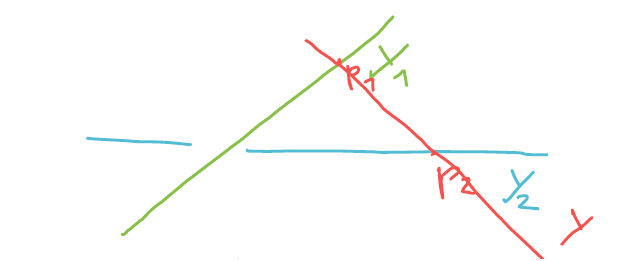
\includegraphics[width=0.5\linewidth]{figures/verbindungsraum_translationen_schnitt_leer}
             \label{fig:verbindungsraum_translationen_schnitt_leer}
         \end{figure}
         Schreibe \( Y_1\vee Y_2=Y_1\vee Y\vee Y_2 \) (verwende dazu \( Y\subseteq Y_1\vee Y_2 \)).
         Verwende \ref{verbindungsraum:translationen:schnitt_nicht_leer} und leite ab, dass gilt:
         \begin{align*}
             T(Y_1\vee Y \vee Y_2)\begin{aligned}[t] 
                 &=T(Y_1)+T(Y\vee Y_2)\\
                 &=T(Y_1)+T(Y)+T(Y_2)\\
                 &=(T(Y_1)+T(Y_2))\needed{\oplus} T(Y).
             \end{aligned}
         \end{align*}
         Es gilt 
         \begin{align*}
             T(Y)=\Set{\lambda\vv{p_1 p_2}| \lambda\in K}.
         \end{align*}
         Wir wollen zeigen
         \begin{align*}
             (T(Y_1)+T(Y_2))\cap T(Y)=\zeroset.
         \end{align*}
         Es genügt zu zeigen
         \begin{align*}
             \vv{p_1 p_2}\notin T(Y_1)+T(Y_2).
         \end{align*}
         Gegenannahme:
         \begin{align*}
             \vv{p_1 p_2}=\underrelate{\vertni}{T(Y_1)}{\vv{p_1 y_1}}+\underrelate{\vertni}{T(Y_2)}{\vv{q_2 p_2}}
         \end{align*}
         mit \( q_1\in Y_1 \), \( q_2\in Y_2 \).
         \begin{figure}[H]
             \centering
             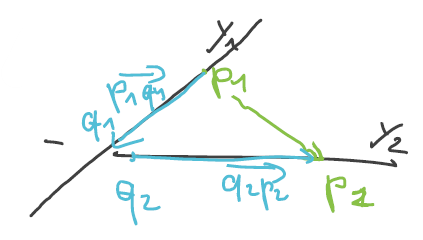
\includegraphics[width=0.5\linewidth]{figures/verbindungsraum_translationen_schnitt_leer_verbindungslinie_nicht_in_translationen}
             \label{fig:verbindungsraum_translationen_schnitt_leer_verbindungslinie_nicht_in_translationen}
         \end{figure}
         Dann gilt
         \begin{align*}
             \vv{q_1 q_2}=\vv{q_1 p_1}+\vv{p_1 p_2}+\vv{p_2 q_2}=0,
         \end{align*}
         also \( q_1=q_2 \) und \( Y_1\cap Y_2\neq \emptyset \) \contra.
    \end{proofdescription}
\end{proof}
Als nächstes: \( \dim(Y_1\vee Y_2) \) ist durch \( \dim_K T(Y_1\vee Y_2) \) gegeben, also sollten wir aus \thref{verbindungsraum:translationen} für \( Y_1\vee Y_2 \) ableiten können.
\begin{lemma}\label{verbindungsraum:dimension}
    Sei \( X \) ein affiner Raum, \( Y_1, Y_2\neq \emptyset \) affine Unterräume von \( X \).
    \begin{eigenschaftenenumerate}
        \item\label{verbindungsraum:dimension:schnitt_nicht_leer} Sei \( Y_1\cap Y_2\neq \emptyset \).
         Dann gilt \( \dim(Y_1\vee Y_2)=\dim(Y_1)+\dim(Y_2)-\dim(Y_1\cap Y_2) \).
        \item\label{verbindungsraum:dimension:schnitt_leer} Sei \( Y_1\cap Y_2=\emptyset \).
        Dann gilt
        \begin{align*}
            \dim(Y_1\vee Y_2)=\dim(Y_1)+\dim(Y_2)-\dim(T(Y_1)\cap T(Y_2))+1.
        \end{align*}
    \end{eigenschaftenenumerate}
    
\end{lemma}
\begin{proof}
    \begin{proofdescription}
        
        \item[\ref{verbindungsraum:dimension:schnitt_nicht_leer}] Aus \thref{verbindungsraum:translationen} folgt
        \begin{align*}
            T(Y_1\vee Y_2)=T(Y_1)+T(Y_2),
        \end{align*}
        aus der Dimensionsformel für Untervektorräume folgt
        \begin{equation*}
            \dim (Y_1\vee Y_2)\begin{aligned}[t] 
                &=\dim T(Y_1\vee Y_2)\\
                &=\dim(Y_1)+\dim T(Y_2)-\dim(T(Y_1)\cap T(Y_2))\\
                &\explain{\text{\thref{schnittraum:translationen}}}{=}\dim T(Y_1)+\dim T(Y_2)-\dim T(Y_1\cap Y_2)\\
                &=\dim Y_1+\dim Y_2-\dim Y_1\cap Y_2.
            \end{aligned}
        \end{equation*}
        
        \item[\ref{verbindungsraum:dimension:schnitt_leer}] \( Y_1\cap Y_2 \), \( p_1\in Y_1 \), \( p_2\in Y_2 \), \( Y=p_1\vee p_2 \).
        
        Dann ist
        \begin{align*}
            \dim Y=\dim T(Y)=1.
        \end{align*}
        Wir erhalten
        \begin{align*}
            \dim (Y_1\vee Y_2)\begin{aligned}[t] 
                &=\dim T(Y_1\vee Y_2)\\
                &\explain{\text{\thref{verbindungsraum:translationen}}}{=}\dim((T(Y_1)+T(Y_2))\oplus T(Y))\\
                &=\dim(T(Y_1)+T(Y_2))+\equalto{1}\dim T(Y)\\
                &=\dim T(Y_1)+\dim T(Y_2)- \dim (T(Y_1)\cap T(Y_2))+1\\
                &=\dim Y_1+\dim Y_2 -\dim(T(Y_1)\cap T(Y_2))+1
            \end{aligned}
        \end{align*}
    \end{proofdescription}
\end{proof}
\begin{beispiel*}[\( X=\reals^3 \)]
    \begin{figure}[H]
        \centering
        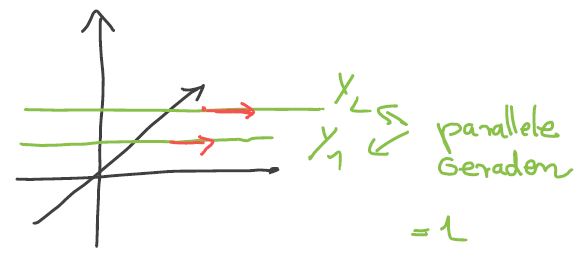
\includegraphics[width=0.5\linewidth]{figures/verbindungsraum_parallele_geraden}
        \label{fig:verbindungsraum_parallele_geraden}
    \end{figure}
    \begin{align*}
        \dim (Y_1\vee Y_2)=1+1-\underbrace{\dim(T(Y_1)\cap T(Y_2))}_{=1}+1=2
    \end{align*}
    \begin{figure}[H]
        \centering
        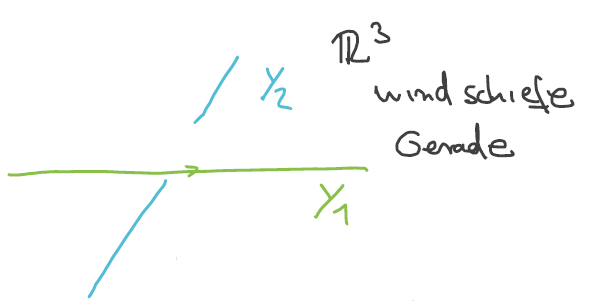
\includegraphics[width=0.6\linewidth]{figures/verbindungsraum_windschiefe_geraden}
        \label{fig:verbindungsraum_windschiefe_geraden}
    \end{figure}
    \begin{align*}
        \dim (Y_1\vee Y_2)1+1-0+1=3
    \end{align*}
    und \( Y_1\vee Y_2=X \).
    
\end{beispiel*}
\section{Parallelprojektionen}
\begin{wiederholung*}[Projektionen aus der \agla{1}]
    \begin{beispiel*}
        \begin{figure}[H]
            \centering
            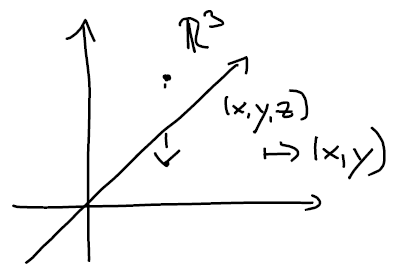
\includegraphics[width=0.5\linewidth]{figures/r_3_projektion}
            \label{fig:r_3_projektion}
        \end{figure}
        
    \end{beispiel*}
    Sei \( V \) ein \( K \)-Vektorraum, \( W, W_1\subset V \) \( K \)-Untervektorräume mit \( V=W\oplus W_1 \).
    Schreibe \( v\in V \) in der Form \( v=w+w_1 \) und mit \( w\in W \), \( w_1\in W_1 \). Definiere
    \begin{align*}
        P_W\maps \begin{aligned}[t] 
            V&\to W_1\\
            \equalto{w+w_1}{v}&\mapsto w_1.
        \end{aligned}
    \end{align*}
    Ein paar Eigenschaften von \( P_W \):
    \begin{itemize}
        \item \( P_W\maps V \to W_1 \) ist eine lineare Abbildung,
        \item \( \Ker P_W=W \),
        \item \( \evaluateat{P_W}{W_1}=\Id_{W_1} \).
    \end{itemize}
    Als Nächstes:
    Wir schränken \( P_W \) ein auf einen Untervektorraum \( W_0 \) von \( V \).
    \begin{figure}[H]
        \centering
        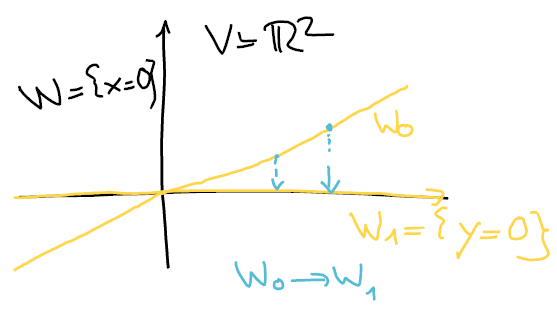
\includegraphics[width=0.5\linewidth]{figures/projektion_einschraenkung_auf_w_0}
        \label{fig:projektion_einschraenkung_auf_w_0}
    \end{figure}
    \begin{lemma}\label{projektion_isomorph}
        Sei \( V \) ein \( K \)-Vektorraum, \( W,W_0, W_1\subseteq V \) Untervektorräume mit \( V=W\oplus W_0=W\oplus W_1 \).

        Dann ist \( \evaluateat{P_W}{W_0}\maps W_0\to W_1 \) ein Isomorphismus (Notation wie oben).
    \end{lemma}
    \begin{proof}
        Es gilt \( \dim W_0=\dim W_1 \) und es genügt zu zeigen, dass \( \evaluateat{P_W}{W_0} \) injektiv ist.

        Sei \( \evaluateat{P_W}{w_0}=w_1 \) für \( w_0\in W_0 \), \( w_1\in W_1 \). Dann ist \( w_0=w+w_1 \) mit \( w\in W \), \( w_1\in W_1 \), also
        \begin{align*}
            w_1=\underrelate{\textcolor{LimeGreen}{\vertni}}{\textcolor{LimeGreen}{W_0}}{w_0}-\underrelate{\textcolor{LimeGreen}{\vertni}}{\textcolor{LimeGreen}{W}}{w}\in W_0\oplus W,
        \end{align*}
        und diese Zerlegung ist eindeutig.
        
    \end{proof}
    
\end{wiederholung*}
\subsection*{Parallelprojektionen für affine Räume}
Sei \( X \) ein affiner Raum (über einem Körper \( K \)), \( Y_1\subseteq X \) ein affiner Unterraum
\begin{beispiel*}
    \begin{figure}[H]
        \centering
        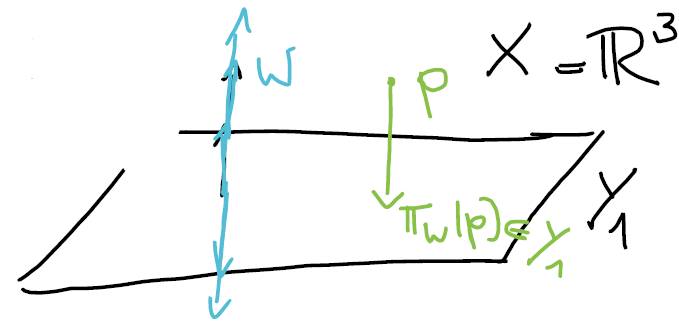
\includegraphics[width=0.5\linewidth]{figures/affine_parallelprojektion_r_3}
        \label{fig:affine_parallelprojektion_r_3}
    \end{figure}
    
\end{beispiel*}
Sei \( W\subseteq T(X) \) ein Untervektorraum mit \( T(X)=T(Y_1)\oplus W \).
\begin{ziel*}
    Definiere eine Projektionsabbildung
    \begin{align*}
        \pi_W\maps X\to Y_1
    \end{align*}
    \enquote{längs \( W \)}.
\end{ziel*}
Für \( p\in X \) definiere
\begin{align*}
    W(p)\definedas\Set{x\in X| \vv{px}\in W}
\end{align*}
\begin{lemma}
    Notation wie oben.
    Für \( p\in X \) gilt
    \begin{align*}
        \anzahl(Y_1\cap W(p))=1.
    \end{align*}
\end{lemma}
\begin{proof}
    Wir berechnen
    \begin{align*}
        \dim(Y_1\cap W(p)).
    \end{align*}
    Sei \( x=\dim X \), verwende \thref{verbindungsraum:dimension}~\ref{verbindungsraum:dimension:schnitt_leer}.
    Falls \( Y_1\cap W(p)=\emptyset \), dann
    \begin{align*}
        \dim(Y_1\vee W(p))\begin{aligned}[t] 
            &=\dim Y_1+\dim W(p)-\dim(\underbrace{T(Y_1)\cap W}_{\textcolor{LimeGreen}{=\zeroset}})+1\\
            &=\dim T(Y_1)+\dim W+1
        \end{aligned}
    \end{align*}
    \contra zu \( Y_1\vee W(p)\subseteq X \), also ist \( Y_1\cap W(p)\neq \zeroset \), und nach \thref{verbindungsraum:dimension}~\ref{verbindungsraum:dimension:schnitt_nicht_leer} gilt Folgendes:
    \begin{align*}
        \equalto{n}{\underbrace{\dim (Y_1\vee W(p))}}\begin{aligned}[t] 
            &=\dim Y_1+\dim W(p)-\dim(Y_1\cap W(p))\\
            &=n-\dim(Y_1\cap W(p))
        \end{aligned}
    \end{align*}
    und nach \thref{schnittraum:translationen}
    \begin{align*}
        \dim Y_1\vee W(p)\begin{aligned}[t] 
            &=\dim(T(Y_1)+W)\\
            &=n,
        \end{aligned}
    \end{align*}
    also \( \dim(Y_1\cap W(p))=0 \).
    
\end{proof}
Wir definieren die Projektion längs \( W \)
\begin{align*}
    \pi_W\maps \underrelate{\subseteq}{Y_0}{X}\to Y_1,\logicspace p\mapsto W(p)\cap Y_1.
\end{align*}
\begin{satz}
    Sei \( X \) ein affiner Raum, \( Y_1,Y_0\subseteq X \) affine Unterräume, \( W\subseteq T(X) \) ein Untervektorraum mit 
    \begin{align*}
        T(X)=W\oplus T(Y_0)=W\oplus T(Y_1).
    \end{align*}
    Dann ist \( \pi_W\maps X\to Y_1 \) eine surjektive affine Abbildung und \( \evaluateat{\pi_w}{Y_0}\maps Y_0\to Y_1 \) eine Affinität.
\end{satz}
\begin{proof}
    Seien \( p,q\in X \).
    \begin{figure}[H]
        \centering
        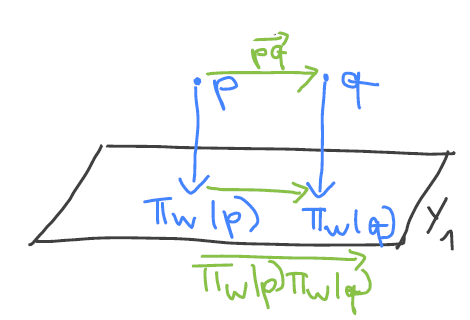
\includegraphics[width=0.5\linewidth]{figures/affine_projektion_ist_affin}
        \label{fig:affine_projektion_ist_affin}
    \end{figure}
    Dann gilt
    \begin{align*}
        \vv{pq}\begin{aligned}[t] 
            &=\vv{p\pi_W(p)}+\vv{\pi_W(p)\pi_W(q)}+\vv{\pi_W(q)q}+\vv{\pi_W(q)q}\\
            &=\underbrace{\vv{p\pi_W(p)}+\vv{\pi_W(q)q}}_{\textcolor{Cyan}{\in W}}+\underbrace{\vv{\pi_W(p)\pi_W(q)}}_{\textcolor{Cyan}{\in T(Y_1)}},
        \end{aligned}
    \end{align*}
    also \( \vv{\pi_W(p)\pi_W(q)}=P_W(\vv{pq}) \).

    \( P_W \) ist surjektiv, also ist \( \pi_W \) eine surjektive affine Abbildung.

    Der zweite Teil folgt aus \thref{projektion_isomorph}.
\end{proof}
% !TEX root = ./Vorlesungsmitschrift AGLA 2.tex  
\lecture{Di 28.04. 10:15}{}
\section{Affine Koordinaten}
Koordinaten in einem \( K \)-Vektorraum \( V \). Sei \( \dim V=n \) und \( v_1,\dotsc , v_n \) eine Basis von \( V \). Dann ist die Abbildung
\begin{align*}
    \phi\maps  \begin{aligned}[t]
        K^n&\to V\\
        (x_1,\dotsc,x_n)&\mapsto \sum\limits_{i=1}^{n}x_i v_i
    \end{aligned}
\end{align*}
ein Isomorphismus von \( K \)-Vektorräumen. Jeder Punkt \( \underrelate{\ni}{V}{v}=\sum_{i=1}^{n}x_i v_i \) ist eindeutig bestimmt durch seine \enquote{Koordinaten}
\begin{align*}
    \inf{\phi}(v)=(x_1,\dotsc,x_n)\in K^n.
\end{align*}
\begin{frage*}
    Sei \( X \) ein affiner Raum über einem Körper \( K \). Können wir auch hier die Lage eines Punkte \( p\in X \) durch Angabe von \enquote{Koordinaten} bezüglich einer \enquote{Basis} beschreibe?
    \begin{figure}[H]
        \centering
        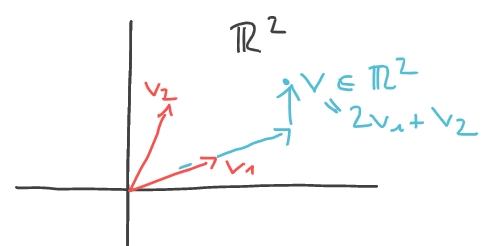
\includegraphics[width=0.5\linewidth]{figures/affine_koordinaten_r_2_hoffnung}
        \label{fig:affine_koordinaten_r_2_hoffnung}
    \end{figure}
    
\end{frage*}
\begin{bspidee*}
    \( X=\reals^2 \) als affiner Raum und Punkte \( p_1,p_2\in X \), sodass \( \vv{p_0p_1} \), \( \vv{p_0p_2} \) eine Basis ist für \( T(X) \). Dann können wir einen Punkt \( p\in X \) beschreiben durch
    \begin{align*}
        p \begin{aligned}[t]
            &=\tau_{\vv{p_0p}}(p_0)\\
            &=\tau_{\lambda\vv{p_0p_1}+\mu\vv{p_0p_2}}(p_0),
        \end{aligned}
    \end{align*}
    falls \( \vv{p_0p}=\lambda\vv{p_0p_1}+\mu\vv{p_0p_2} \) mit \( \lambda,\mu\in \reals \).

    \begin{figure}[H]
        \centering
        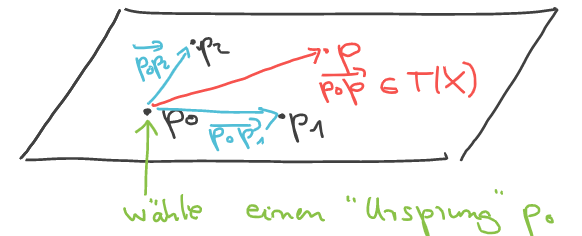
\includegraphics[width=0.5\linewidth]{figures/ursprungswahl}
        \label{fig:ursprungswahl}
    \end{figure}
    
    Wir erhalten eine Abbildung 
    \begin{align*}
        \phi\maps \begin{aligned}[t]
            \reals^2&\to X\\
            (\lambda,\mu)&\mapsto \tau_{\lambda\vv{p_0 p_1}+\mu\vv{p_0 p_2}}(p_0),
        \end{aligned}
    \end{align*}
    die eine Affinität ist.
\end{bspidee*}
Wir formalisieren diese Konzepte für allgemeine affine Räume.
\begin{definition*}
    Sei \( X \) ein affiner Raum und \( p_0,\dotsc, p_n\in X \). Wir nennen \( (p_0,\dotsc,p_n) \) \emph{affin unabhängig} \bzw eine \emph{affine Basis}, wenn die Vektoren \( (\vv{p_0p_1},\dotsc, \vv{p_0p_n}) \) in \( T(x) \) \emph{linear unabhängig sind} \bzw \emph{eine Basis bilden}.
\end{definition*}
\begin{beispiele*}
    \begin{enumerate}
        \item In \( X=\reals^n \) ist \( (0,e_1,\dotsc, e_n) \) eine affine Basis.
        \item \( X=\reals^n \) als affiner Raum, \( v_1,\dotsc, v_k\in \reals^n \) linear unabhängig, \( v_0=0 \). Dann ist das Tupel \( (v_0,v_1,\dotsc,v_k) \) affin unabhängig.
        \begin{frage*}
            Kann man hier \( v_0\in \reals^n \) beliebig nehmen?
        \end{frage*}
        \item \( X=\reals^2 \) als affiner Raum. Dann gilt, dass für \( v,w\in \reals^2 \) das Tupel \( (v,w) \) affin unabhängig ist \gdw \( v\neq w \).
        \item \( X \) affiner Raum, \( p_0\in X \), \( (t_1,\dotsc,t_n) \) Basis von \( T(X) \). Dann ist
        \begin{align*}
            (p_0,\tau_{t_1}(p_0),\dotsc, \tau_{t_n}(p_0))
        \end{align*}
        eine affine Basis von \( X \).
    \end{enumerate}
    
\end{beispiele*}
\begin{lemma}
    Sei \( X \) ein affiner Raum, \( p_0,\dotsc, p_n\in X \) und \( (p_0,\dotsc, p_n) \) affin unabhängig. Sei \( \sigma\in S_{n+1} \) eine Permutation von \( \Set{0,\dotsc,n} \). Dann ist
    \begin{align*}
        (p_{\sigma(0)},p_{\sigma(1)},\dotsc,p_{\sigma(n)})
    \end{align*}
    affin unabhängig.
\end{lemma}
\begin{proof}
    Wir wollen zeigen, dass unter den Annahmen des Lemmas, die Vektoren
    \begin{align*}
        \vv{p_{\sigma(0)}p_{\sigma(1)}},\dotsc,\vv{p_{\sigma(0)p_{\sigma(n)}}}\in T(X)
    \end{align*}
    linear unabhängig sind.

    Sei \( \sigma(0)=i\in \Set{0,\dotsc,n} \).

    Dann müssen wir also zeigen, dass die Vektoren
    \begin{align*}
        \vv{p_i p_0},\vv{p_i p_1},\dotsc, \vv{p_i p_{i-1}},\vv{p_i p_{i+1}},\dotsc,\vv{p_i p_n}
    \end{align*}
    linear unabhängig sind.

    Seien \( \lambda_0,\dotsc, \lambda_{i-1},\lambda_{i+1},\dotsc,\lambda_n\in K \) mit
    \begin{align*}
        \lambda_0 \vv{p_i p_0}+\lambda_1\vv{p_i p_1}+\dotsb+\lambda_{i-1}\vv{p_i p_{i-1}}+\lambda_{i+1}\vv{p_i p_{i+1}}+\dotsb+\lambda_n\vv{p_i p_n}=0.
    \end{align*}
    Schreibe
    \begin{align*}
        \vv{p_i p_j}=\vv{p_i p_0}+\vv{p_0 p_j}=\textcolor{Goldenrod}{\vv{p_0 p_j}}-\textcolor{LimeGreen}{\vv{p_0 p_i}}.
    \end{align*}
    Wir erhalten
    \begin{align*}
        \begin{aligned}[t]
            \textcolor{Goldenrod}{\lambda_1\vv{p_0 p_1}+\dotsb+\lambda_{i-1} \vv{p_0 p_{i-1}}+\lambda_{i+1} \vv{p_0 p_{i+1}}+\dotsb+\lambda_n \vv{p_0 p_n}}\\
            -\textcolor{LimeGreen}{(\lambda_0+\dotsb+\lambda_{i-1}+\lambda_{i+1}+\dotsb+\lambda_n)\vv{p_0 p_i}}=0
        \end{aligned}
    \end{align*}
    Aus der linearen Unabhängigkeit von \( \vv{p_0 p_1},\dotsc, \vv{p_0 p_n} \) folgt
    \begin{align*}
        \lambda_1=\dotsb=\lambda_{i-1}=\lambda_{i+1}=\lambda_n=0
    \end{align*}
    und
    \begin{align*}
            \explain{\lambda_0=0}+\underbrace{\lambda_1+\dotsb+\lambda_{i-1}+\lambda_{i+1}+\dotsb+\lambda_n}_{=0}=0
    \end{align*}
\end{proof}
\subsection*{Affine Basen und affine Abbildungen}
Aus der AGLA \Romannum{1}:\\
Seien \( V,W \) \( K \)-Vektorräume, \( v_1,\dotsc, v_n \in V \) eine Basis von \( V \) und \( w_1,\dotsc, w_n \in W\). Dann gibt es genau eine \( K \)-lineare Abbildung \( \phi\maps V\to W \) mit
\begin{align*}
    \phi(v_i)=w_i,\quad 1\leq i \leq n.
\end{align*}
\begin{figure}[H]
    \centering
    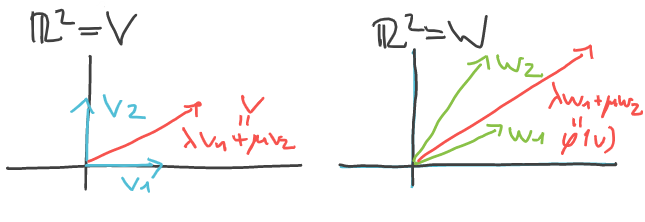
\includegraphics[width=0.7\linewidth]{figures/bilder_der_basen_bestimmt_abbildung_r_2}
    \label{fig:bilder_der_basen_bestimmt_abbildung_r_2}
\end{figure}
\begin{frage*}
    Inwiefern sind affine Abbildungen zwischen affinen Räumen durch die Bilder einer affinen Basis bestimmt?
\end{frage*}
\begin{satz}\label{bilder_der_basen_bestimmen_affine_abbildung}
    Seien \( X,Y \) affine Räume, \( (p_0,\dotsc,p_n) \) eine affine Basis von \( X \) und \( q_0,\dotsc, q_n\in Y \). Dann gibt es genau eine affine Abbildung \( f\maps X\to Y \) mit
    \begin{align*}
        f(p_i)=q_i,\quad 0\leq i\leq n.
    \end{align*}
    Die Abbildung \( f \) ist \emph{injektiv} \bzw \emph{eine Affinität} \gdw das Tupel \( (q_0,\dotsc, q_n) \) \emph{affin unabhängig} \bzw \emph{eine affine Basis} von \( Y \) ist.
\end{satz}
\begin{proof}
    Eine affine Abbildung \( f\maps X\to Y \) ist gegeben durch \( f(p_0) \) für ein \( p_0\in X \) und eine lineare Abbildung
    \begin{align*}
        F\maps \begin{aligned}[t]
            T(X)&\to T(Y)\\
            \vv{pq}&\mapsto \vv{f(p)f(q)}.
        \end{aligned}
    \end{align*}
    Wir definieren \( F \) durch
    \begin{align*}
        F(\vv{p_0 p_i})=\vv{q_0 q_i}\quad 1\leq i \leq n. \tag{*}\label{bilder_der_basen_bestimmt_affine_abbildung:beweis:k_lineare_abbildung}
    \end{align*}
    \( \vv{p_0 p_1}, \dotsc, \vv{p_0 p_n} \) ist eine Basis von \( T(X) \), also gibt es genau ein lineare Abbildung
    \begin{align*}
        F\maps T(X)\to T(Y)
    \end{align*}
    mit \eqref{bilder_der_basen_bestimmt_affine_abbildung:beweis:k_lineare_abbildung}. Es gilt dann
    \begin{align*}
        f(p_i)\begin{aligned}[t]
            &=\tau_{\vv{f(p_0) f(p_i)}} f(p_0)\\
            &=\tau_{F(\vv{p_0 p_i})} f(p_0)\\
            &=\tau_{\vv{q_0 q_i}} q_0 =q_i \quad 1\leq i \leq n.
        \end{aligned}
    \end{align*}
    \( f \) ist injektiv \gdw \( F \) injektiv ist. \( F \) ist injektiv \gdw \( \vv{q_0 q_1}, \dotsc, \vv{q_0 q_n} \) linear unabhängig sind.

    \tto \( f \) ist eine Affinität \gdw \( F \) bijektiv ist. \( F \) ist bijektiv \gdw \( \vv{q_0 q_1}, \dotsc, \vv{q_0 q_n} \) eine Basis von \( T(Y) \) ist.

\end{proof}
\subsection*{Affine Koordinatensysteme}
Sei \( X \) ein affiner Raum über einem Körper \( K \), \( (p_0,p_1,\dotsc, p_n) \) eine affine Basis von \( X \).

Nach \thref{bilder_der_basen_bestimmen_affine_abbildung} gibt es genau eine Affinität
\begin{align*}
    \phi\maps K^n\to X
\end{align*}
mit \( \phi(0)=p_0, \phi(e_1)=p_1,\dotsc, \phi(e_n)=p_n \) und zugehörige lineare Abbildung \( \Phi\maps K^n \to T(X) \).

Einen Punkt \( p\in X \) können wir dann beschreiben durch
\begin{align*}
    p=\tau_{\vv{p_0 p}}(p_0).
\end{align*}
Sei \( \vv{p_0 p}=\lambda_1 \vv{p_0 p_1}+\dotsb +\lambda_n \vv{p_0 p_n} \) mit \( \lambda_i\in K \), \( 1\leq i \leq n \).

Dann ist
\begin{align*}
    p \begin{aligned}[t]
        &=\tau_{\lambda_1\vv{p_0 p_1}+\dotsb +\lambda_n\vv{p_0 p_n}}(p_0)\\
        &=\tau_{\lambda_1 \Phi(e_1)+\dotsb+\lambda_n \Phi(e_n)}(p_0)\\
        &=\tau_{\Phi(\lambda_1 e_1+\dotsb+\lambda_n e_n)}(p_0),
    \end{aligned}
\end{align*}
oder \( p=\phi((\lambda_1,\dotsc,\lambda_n)) \).

\begin{definition*}
    Sei \( X \) ein affiner Raum über einem Körper \( K \). Wir nennen eine Affinität \( \phi\maps K^n\to X \) ein affines Koordinatensystem in \( X \). Seu \( p_0=\phi(0),p_1=\phi(e_1),\dotsc, p_n=\phi(e_n) \). Dann ist \( (p_0,\dotsc,p_n) \) eine affine Basis von \( X \).

    Für \( p\in X \) nennen wir
    \begin{align*}
        \inv{\phi}(p)=(x_1,\dotsc,x_n)\in K^n
    \end{align*}
    den Koordinatenvektor von \( p \) bezüglich der affinen Basis \( (p_0,\dotsc,p_n) \) und \( (x_1,\dotsc, x_n) \) die Koordinaten von \( p \) bezüglich \( (p_0,\dotsc, p_n) \).
    \begin{figure}[H]
        \centering
        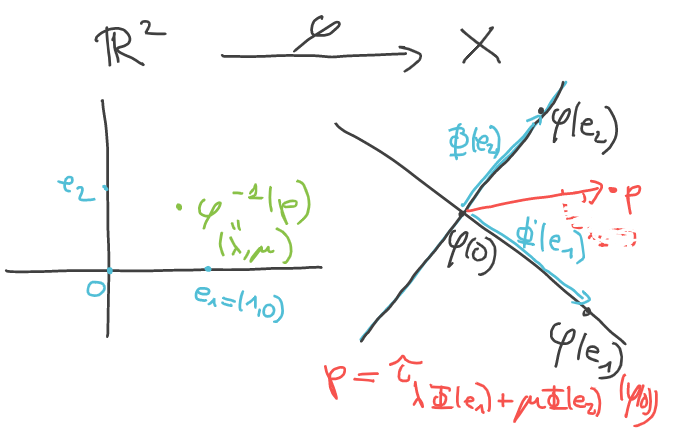
\includegraphics[width=0.7\linewidth]{figures/affine_koordinatenabbildung_r_2}
        \label{fig:affine_koordinatenabbildung_r_2}
    \end{figure}
\end{definition*}
\section{Das Teilverhältnis}
\begin{idee*}
    Seien 3 Punkte \( p_0,p_1,p \) auf einer Gerade \( l \) (\zb im \( \reals^3 \)) gegeben, \( p_0\neq p_1 \).
    \begin{figure}[H]
        \centering
        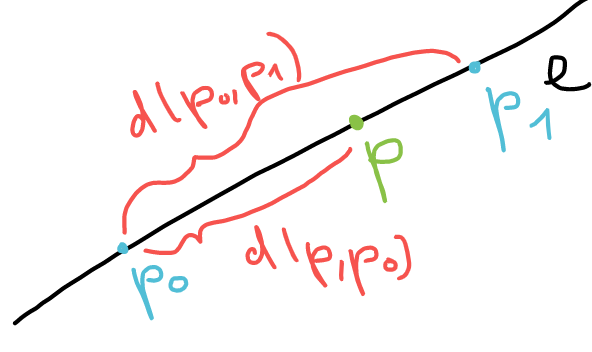
\includegraphics[width=0.5\linewidth]{figures/gerade_teilverhaeltnis}
        \caption*{}
        \label{fig:gerade_teilverhaeltnis}
    \end{figure}
    Sei \( \lambda=\frac{d(p,p_0)}{d(p_1,p_0)} \), mit \( d \) dem euklidischen Abstand, dann können wir die Lage von \( p \) auf \( l \) durch \( \lambda \) (und der Information, ob \( p \) \enquote{rechts oder links} von \( p \) liegt) bestimmen.
\end{idee*}
\begin{definition*}
    Sei \( X \) ein affiner Raum über \( K \), \( Y\subseteq X \) eine affine Gerade, \( p_0,p_1,p\in Y \) und \( p_0\neq p_1 \). Dann nennen wir das eindeutig bestimmte Element \( \lambda\in K \) mit \( \vv{p_0 p}=\lambda \vv{p_0 p_1} \) das Teilverhältnis von \( p_0,p_1,p \). Schreibe \( \lambda=\teilverhaeltnis(p_0,p_1,p) \). In \( \characteristic(K)\neq 2 \) nennen wir \( p \) Mittelpunkt von \( p_0,p_2 \) wenn \( \teilverhaeltnis(p_0,p_1,p)=\frac{1}{2} \).
\end{definition*}
\begin{bemerkungen*}
    \begin{enumerate}
        \item Es gilt \( T(Y)=K\vv{p_0p_1} \). Damit ist \( \lambda \) wohldefiniert und existiert.
        \item \( p_0,p_1 \) ist eine affine Basis von \( Y \). Damit existiert ein Koordinatensystem
        \begin{align*}
            \phi\maps K\to Y,\logicspace \begin{aligned}[t]
                \phi(0)&=p_0\\
                \phi(1)&=p_1
            \end{aligned}
        \end{align*}
        und es gilt \( \teilverhaeltnis(p_0,p_1,p)=\inv{\phi(p)} \).
    \end{enumerate}
    
\end{bemerkungen*}
\begin{frage*}
    Wie verhält sich das Teilverhältnis unter affinen Abbildungen?
    \begin{figure}[H]
        \centering
        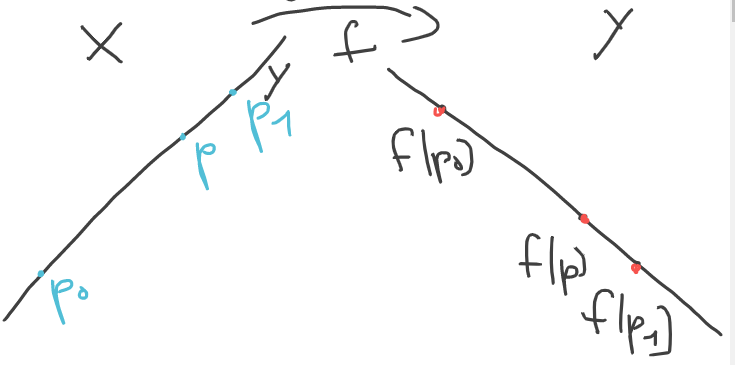
\includegraphics[width=0.7\linewidth]{figures/affine_abbildungen_wirkung_auf_teilverhaeltnis}
        \label{fig:affine_abbildungen_wirkung_auf_teilverhaeltnis}
    \end{figure}
    
\end{frage*}

\begin{lemma}\label{teilverhaeltnis_invariant_unter_affinen_abbildungen}
    Seien \( X,Y \) affine Räume und \( f\maps X\to Y \) eine affine Abbildung, seien \( p_0,p1,p \) Punkte in \( X \), die auf einer Geraden liegen und \( f(p_0)\neq f(p_1) \). Dann gilt
    \begin{align*}
        \teilverhaeltnis(f(p_0),f(p_1),f(p))=\teilverhaeltnis(p_0,p_1,p).
    \end{align*}
\end{lemma}
\begin{proof}
    Sei \( \lambda=\teilverhaeltnis(p_0,p_1,p) \), also \( \vv{p_0 p}=\lambda\vv{p_0 p_1} \). Si \( F\maps T(X)\to T(Y) \) die zu \( f \) gehörige lineare Abbildung. Wir berechnen
    \begin{align*}
        \vv{f(p_0) f(p)}\begin{aligned}[t]
            &=F(\vv{p_0 p})\\
            &=F(\lambda{p_0 p_1})\\
            &=\lambda F({p_0 p_1})\\
            &=\lambda \vv{f(p_0) f(p_1)}
        \end{aligned}
    \end{align*}
    
\end{proof}
\begin{anwendung*}[Strahlensatz]
    Sei \( X \) ein affiner Raum über \( K \), \( p_0,p_1,p_2\in X \) affin unabhängig. Sei
    \begin{align*}
        q_1&\in p_0\vee p_1,\logicspace q_1\neq p_0\\
        q_2&\in p_0\vee p_2,\logicspace q_2\neq p_0.
    \end{align*}
    Wir nehmen an, dass \( p_1\vee p_2 \) und \( q_1\vee q_2 \) parallel sind in dem Sinn, dass
    \begin{align*}
        T(p_1\vee p_2)=T(q_1\vee q_2)\text{ in }T(X).
    \end{align*}
    Dann gilt
    \begin{align*}
        \teilverhaeltnis(p_0,p_1,q_1)=\teilverhaeltnis(p_0,p_2,q_2).
    \end{align*}
    \begin{figure}[H]
        \centering
        \includegraphics[width=0.5\linewidth]{figures/Strahlensatz}
        \label{fig:Strahlensatz}
    \end{figure}
\end{anwendung*}
\begin{proof}
    Sei \( Y \) diedurch \( p_0,p_1,p_2 \) aufgespannte Ebene. Dann gibt es ein affines Koordinatensystem \( \phi\maps K^2 \to Y \) mit \( \phi(0)=p_0, \phi(e_1)=p_1, \phi(e_2)=p_2 \).
    \begin{figure}[H]
        \centering
        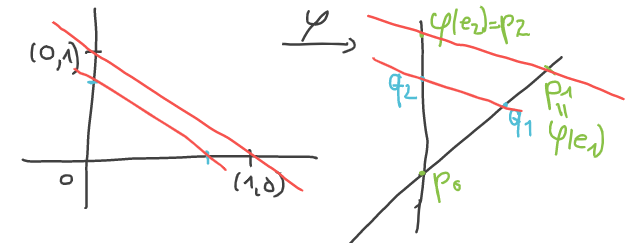
\includegraphics[width=0.5\linewidth]{figures/strahlensatz_koordinatensystem}
        \label{fig:strahlensatz_koordinatensystem}
    \end{figure}
    Sei
    \begin{align*}
        (\lambda,0)&=\inv{\phi}(q_1)\\
        (0,\mu)&=\inv{\phi}(q_2).
    \end{align*}    
    \begin{behauptung*}
        \( l_1=\inv{\phi}(q_1)\vee \inv{\phi}(q_2) \) und \( l_2=\inv{\phi}(p_1)\vee \inv{\phi}(p_2) \) sind parallel.
    \end{behauptung*}
    \minisec{Denn:}
    \begin{align*}
        T(l_1)&=K\vv{\inv{\phi}(q_1) \inv{\phi}(q_2)}\\
        T(l_2)&=K\vv{\inv{\phi}(p_1) \inv{\phi}(p_2)}.
    \end{align*}
    Es ist \( K\vv{p_1 p_2}=K\vv{q_1 q_2} \) und daher
    \begin{align*}
        \equalto{K\vv{\inv{\phi}(q_1) \inv{\phi}(q_2)}}{K \inv{\Phi}(\vv{p_1 p_2})}=\equalto{K\vv{\inv{\phi}(p_1) \inv{\phi}(p_2)}}{K\inv{\Phi}(\vv{q_1 q_2}}).
    \end{align*}
    Aus der Parallelität von \( l_1,l_2 \) folgt \( \lambda=\mu \).

    Also
    \begin{align*}
        &\rphantom{=}\teilverhaeltnis(\inv{\phi}(p_0),\inv{\phi}(p_1),\inv{\phi}(q_1))=\lambda\\
        &=\mu=\teilverhaeltnis(\inv{\phi}(p_0),\inv{\phi}(p_2),\inv{\phi}(q_2))
    \end{align*}
    und der Strahlensatz folgt aus \thref{teilverhaeltnis_invariant_unter_affinen_abbildungen}.
\end{proof}


% End of lectures

\end{document}
